\documentclass[12pt]{article}
\title{Project Interviews}
\author{Bertagnoli Daniele 1903768 \\ Costantino Giuseppe 1677800 \\ Frascarelli Giacomo 1917888 \\ Guarino Marco 1895383}
\date{2023/2024}

\usepackage[left=2cm, right=2cm]{geometry}
\usepackage{amsmath}
\usepackage{graphicx}
\usepackage{subfig}
\usepackage{hyperref}

\begin{document}
\maketitle

\tableofcontents
\newpage

\section{Interviews}

\subsection{Questions}
These interviews were conducted to assess the viability of the project idea and serve as the initial stage of the need-finding process. The questions asked to the participants during the interview are:
\begin{enumerate}
    \item Have you experienced situations in which you or someone you know was in danger? (e.g., my father fell down and was not able to use the phone) If yes, what was the situation? Were you able to contact someone for help? Was it difficult, or were you able to alert someone easily?
    \item Would you install the application to alert contacts in an easy and fast way? Do you find this idea useful?
    \item Do you prefer to inform contacts through a phone call, SMS, or a notification? (Or other options)
    \item Would you install such an application to be informed about other contacts' emergencies? Why?
\end{enumerate}

\subsection{Answers}
The following rows contain the main content of each interview, 
highlighting the most significant contributions given by each participant:

\begin{enumerate}
    \item She said that once her grandmother had a medical emergency at 
    home, and she wasn't able to reach anyone for help because her phone 
    was out of reach. However, the grandmother is not able to use the 
    smartphone.
    
    \item He shared a story about a camping trip where one of his friends got 
    injured, and his phone fell several meters away from him. He started screaming 
    to ask for help, luckily, the other friends heard him. He said that he would 
    install that application only during particular periods of the year, such as when 
    he goes on holidays during summer. He prefers phone calls whenever possible.
    
    \item He mentioned a situation where a colleague experienced a severe allergic 
    reaction while he was alone at home. He was able to use the phone, but he 
    struggled to talk during the phone call with the ambulance operators. He said 
    that probably a method to alert family members in some ways with predefined 
    messages was probably the best thing in that situation because he had to alert 
    them several hours later when the crisis was gone. He told us that these 
    situations are not so common, so probably he wouldn't install such an application 
    as he prefers to be contacted via WhatsApp or SMS through that system.
    
    \item She told us about one situation in which she felt followed by someone. 
    Because she was very nervous, she had some difficulties quickly dialing her 
    mother's phone number on the phone. She stated that she would install the 
    application to feel safer when she comes back home during late hours of the day.
    
    \item He doesn't know anyone who experienced emergencies. He said that this is a 
    situation he has never thought about, but the application could be useful for his 
    grandma who lives alone and uses a smartphone. The interviewee prefers to be 
    informed via notifications.

    \item She said her mother fell to the ground in the evening, couldn't 
    get up, and couldn't call anyone. She would install an application that 
    could help herself and others in difficult situations. She 
    would like to be notified both by a call and by an SMS.
    
    \item She says she was alone in the middle of the night in Rome and felt 
    like someone was chasing her. So, she was on the phone the whole time 
    with her friend. She would like an application that can promptly assist 
    her in case of difficulty with a call. Additionally, she would install the 
    application to help other people in emergency situations.
    
    \item He has never experienced firsthand situations where he was in trouble 
    or where someone he knows alerted him in emergencies, but he would still 
    find an application for such purposes useful and would install it. 
    He would like to be notified, and to notify others, using all available 
    methods.
    
    \item He experienced a situation where his father had a heart attack 
    and fortunately managed to contact the ambulance but couldn't reach 
    his son, who only found out about the news after some time. So, he 
    would appreciate having the possibility of being contacted immediately. 
    He would thus install the application both in case he himself is in 
    danger and in case it's one of his parents. He would like to be 
    informed with a call and a notification of the location.
    
    \item She has never experienced situations of danger herself nor 
    secondhand where it was necessary to contact someone, but she would 
    appreciate an application that can alert others in a simplified way, 
    and to be alerted, in cases of danger and emergency. She would find it 
    useful to be notified in all available ways, through calls, SMS, and 
    notifications. She would install the application both for herself and 
    for friends or relatives.

    \item The interviewee had a nasty situation once while riding his bike. 
    He slipped while making a turn, and his smartphone flew out of his pocket. 
    Both his legs were stuck underneath the bike, and he was unable to move. 
    It wasn't until a good samaritan came by that he received medical 
    attention. He mentioned that had it been an isolated road with bad 
    weather, he could have easily died that day. He thinks calls are the 
    most effective way to get someone's attention, though a very loud 
    notification from the app could also work. He expressed interest in 
    using the app because his parents are getting older, and he would love 
    to keep an eye on them to be notified immediately in case of an 
    emergency.

    \item This person recounted an incident where she was trying to get her 
    grandfather to bed when he suddenly lost consciousness and fell on his 
    back. She immediately called the emergency number and got him escorted 
    to the hospital. She noted that her grandfather does not even have a 
    clamshell phone and is not keen on integrating technology into his 
    daily life. Thus, she does not think this idea could benefit her 
    family.

    \item She has had a few close calls while rock climbing. One time, she 
    fell and got stuck in a narrow crevice. A fellow climber nearby was able 
    to pull her out safely. This experience made her realize the importance 
    of a reliable emergency response system. She believes this idea could 
    benefit people with disabilities or mobility issues by providing an easy 
    way to alert contacts in case of an emergency. She thinks SMS messages 
    would be the most effective notification method to ensure the person 
    receiving the message is aware of the situation. She would definitely 
    install an app like this to keep an eye on loved ones who live far away, 
    understanding the importance of seniors having autonomy while still 
    having a safety net.

    \item He shared that his mum once fell down the stairs, which was quite 
    worrying for him and his brother. They managed to patch her up, and she 
    walked away with a minor scratch. While he finds the idea useful, he 
    does not trust technology enough. He worries about the phone's battery 
    running out, lack of signal, or a bug preventing a notification from 
    appearing. He prefers good old-fashioned phone calls and does not 
    believe apps can truly benefit daily life.

    \item The interviewee has never had a personal experience with danger 
    but has worked in emergency services for years. He has seen the impact 
    of timely interventions on people's lives, with one incident involving a 
    distress call from a lost hiker. He managed to locate and guide the 
    hiker back to safety, which highlighted the importance of having the 
    right tools and systems in place. He believes efficient communication is 
    crucial and views the app as a game-changer for staying connected and 
    getting help quickly. He thinks a combination of notifications and phone 
    calls would be most effective for alerting contacts in an emergency. 
    He would install the app to receive notifications about other contacts' 
    emergencies, believing in the importance of being connected and informed 
    to help each other, whether by providing support or offering a listening 
    ear.

    \item He recalled a time when his neighbor suffered a stroke while 
    gardening in the backyard. The neighbor's wife was inside the house 
    and unaware of the situation for several minutes. He believes an app 
    that could send alerts through loud notifications would be extremely 
    useful. He prefers SMS and notifications over calls, as they are less 
    intrusive but still effective. He would install the app to ensure his 
    family is informed in case of emergencies.

    \item She shared an incident where she was in a car accident and her 
    phone was damaged, making it impossible to call for help. A passerby 
    assisted her, but the experience made her realize the importance of 
    an emergency alert system. She would definitely install the app, 
    especially for her children who are often away at college. She 
    prefers notifications and SMS for their reliability and simplicity.

    \item He described a situation where his diabetic friend experienced 
    a severe hypoglycemic episode and couldn't reach his phone to call 
    for help. Another friend luckily noticed in time and assisted him. 
    He thinks the app would be beneficial, particularly for people with 
    medical conditions. He prefers notifications as the primary method 
    of alert. He would install the app to monitor his friend's condition 
    and ensure timely assistance.

    \item She mentioned an instance where her elderly father wandered 
    off and got lost while she was at work. It took hours to find him, 
    causing significant distress. She believes an app with GPS tracking 
    and emergency alerts could prevent such situations. She prefers phone 
    calls for immediate attention. She would install the app to keep 
    track of her father's whereabouts and ensure his safety.

    \item He recounted a time when he was hiking alone and twisted
    his ankle, making it difficult to move. His phone signal was weak, 
    and it took a long time to contact anyone for help. He believes an 
    emergency alert app that works in low-signal areas would be 
    invaluable. He prefers SMS for its reliability in such situations. 
    He would install the app for personal safety during solo outdoor 
    activities.

\end{enumerate}

\subsection{Interviews Analysis}
The interviews conducted provided valuable insights into the potential 
viability and usefulness of an emergency alert application. Participants 
shared a diverse range of experiences and opinions, highlighting both the
demand for such a solution and the considerations necessary for its 
successful implementation. There was a significant interest in the 
application among the participants, especially those who had encountered 
emergencies or had elderly family members living alone.

These intereviews underline a common theme: emergencies can occur 
unexpectedly, this highlights a clear need for an application 
that can facilitate quick and easy communication during such critical 
moments.

Preferences for notification methods varied among participants. 
Some preferred phone calls for their immediacy and effectiveness in 
grabbing attention during emergencies. Others favored SMS or app 
notifications, considering them more reliable and less intrusive. 

\section{Questionnaire}
For performing a more extended need-finding phase, we create a Google form 
with some questions to retrieve more information about our idea. The form 
is available at the following link: \url{https://forms.gle/1AnJ6wdFpiuWXPuFA}.

\subsection{Results}
We achieved a total of 80 answers and these are the results. As shown in 
\hyperref[fig:age]{Figure~\ref*{fig:age}}, more than $70\%$ of the partecipants
were having an age between 18 and 30 years old. 

\begin{figure}[ht]
    \centering
    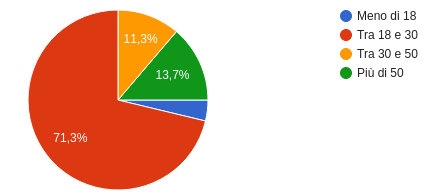
\includegraphics[width=.5\textwidth]{Images/age.png}
    \caption{Graph showing the partecipants' age.}
    \label{fig:age}
\end{figure}

From the second question, we can see how many participants have ever 
been in an emergency situation. $41.3\%$ have never experienced a 
critical situation, while $59.7\%$ have at least one experience. 
As we can see from \hyperref[fig:emergency_user]{Figure~\ref*{fig:emergency_user}},
only $16.3\%$ of the users were not able to alert someone during these 
situations. However, by taking a look at the next question, where the users 
described their experiences, we can see how most of these situations 
could generate so much panic that the user is not able to make quick 
decisions and thus even alerting someone using the phone can be difficult.

\begin{figure}[ht]
    \centering
    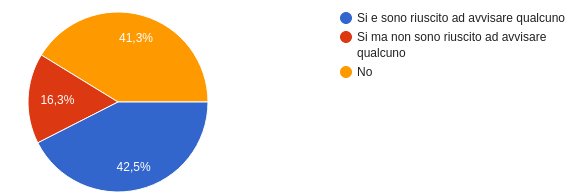
\includegraphics[width=.7\textwidth]{Images/emergency_user.png}
    \caption{Graph showing if the participants have ever experienced
    an emergency situation, and if they were able to alert someone.}
    \label{fig:emergency_user}
\end{figure}

The next two questions are very similar to the previous two. Nevertheless, 
in this case, the users were asked to answer if one of their acquaintances
has ever experienced one of these situations. Unlike the previous 
question, in this case $63.7\%$ of the participants answered 
"No" (\hyperref[fig:emergency_acquaintances]{Figure~\ref*{fig:emergency_acquaintances}}). 
If we look at the open answers, we can see how the experiences
are mostly similar to those described for personal experiences.

\begin{figure}[ht]
    \centering
    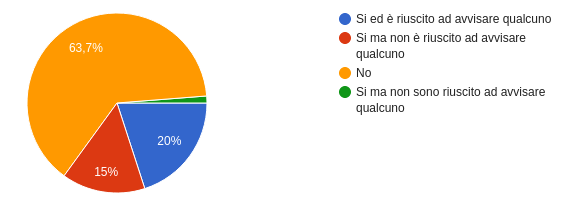
\includegraphics[width=.7\textwidth]{Images/emergency_acquaintances.png}
    \caption{Graph showing if the participants know someone who has ever 
    experienced an emergency situation, and if they were able to alert 
    someone.}
    \label{fig:emergency_acquaintances}
\end{figure}

The motivation most people give for using the app is that it makes the user save precious time.
The arguments being that if someone is injured, panic might prevent the user from making a swift
call to the emergency services.
Even worse, if someone is unable to use their cellphone due to severe injuries or fainting, users suggest
the app could help save their lives.
Other people argue that by intergrating the app with official first response services might result in
a quicker response time (\hyperref[fig:install_for_me]{Figure~\ref*{fig:install_for_me}}).

\begin{figure}[ht]
    \centering
    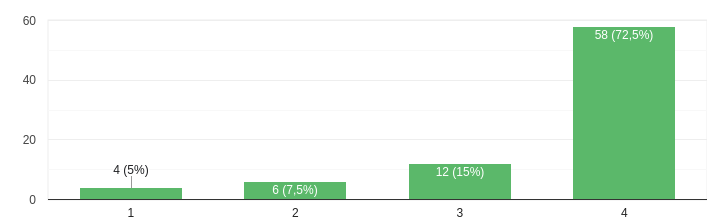
\includegraphics[width=.7\textwidth]{Images/install_for_me.png}
    \caption{Graph showing how the user will likely install the application
    for alerting their contacts.}
    \label{fig:install_for_me}
\end{figure}

A striking majority ($66.3\%$) of people would very surely install the applicaton (4)
followed by $21.3\%$ on option (3), $10.0\%$ on (2), which are not very convinced by the idea,
and lastly $2.5\%$ say they would not install the app.
Overall the response is positive and very encouraging.
(\hyperref[fig:install_for_others]{Figure~\ref*{fig:install_for_others}}).

\begin{figure}[ht]
    \centering
    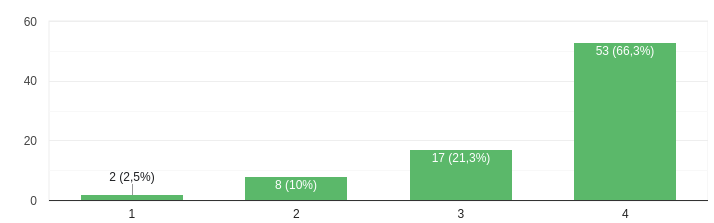
\includegraphics[width=.7\textwidth]{Images/install_for_others.png}
    \caption{Graph showing how the user will likely install the application
    for receiving alerts from their contacts.}
    \label{fig:install_for_others}
\end{figure}

More than half the people ($52.5\%$) would like to be informed by a notification
with relevant infos, followed by $30.0\%$ which would prefer to start an automatic
call to the person in potential danger, and lastly, with $16.3\%$ would prefer an SMS 
(\hyperref[fig:alert_me]{Figure~\ref*{fig:alert_me}}).

\begin{figure}[ht]
    \centering
    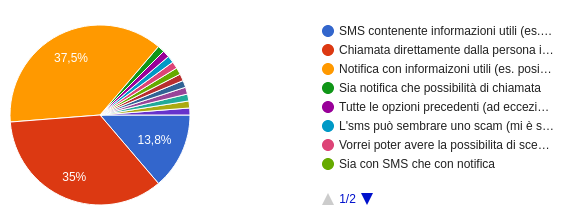
\includegraphics[width=.7\textwidth]{Images/alert_me.png}
    \caption{Graph showing how users want to be alerted.}
    \label{fig:alert_me}
\end{figure}

As for the mean through which people prefer to inform their contacts,
the majority ($37.5\%$) leans towards a notification with important informations.
Followed by an automatic call to a pre-determined contact ($35.0\%$) and lastly SMS 
to pre-determined contact (\hyperref[fig:alert_others]{Figure~\ref*{fig:alert_others}}).

\begin{figure}[ht]
    \centering
    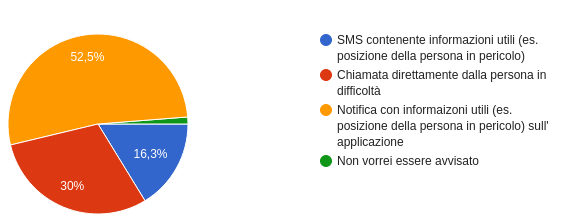
\includegraphics[width=.7\textwidth]{Images/alert_others.png}
    \caption{Graph showing how users want to alert their contacts.}
    \label{fig:alert_others}
\end{figure}

\section{Needs, Context and Interaction Analysis}
\subsection{User's Needs \& Competitors}
After the interviews and the questionnaire, we dedicated a good amount of time to analyze the results, trying to underline the user needs we found through the need-finding step. On Google Play and Apple Store, we didn't find any application with the same intent as the one we tried to propose. There are some applications dedicated to emergencies, but their main scope is to alert ambulances, hospitals, or the police. Our main idea is to create an application to alert someone from our contact list and eventually ambulances. Users don't necessarily need to alert hospitals for their emergencies, so we have to give them the possibility to contact someone and, if needed, the public services. The main goals of our application are:
\begin{itemize}
    \item Keep the interface simple to facilitate usage during emergencies.
    \item Keep the user informed about all the running services, also giving the possibility to turn them off if not needed.
    \item Try to keep only essential background services to avoid energy waste, thus saving phone battery life.
    \item Provide a fast and easy way to use the functionalities even in eye-free situations.
    \item Try to detect specific contexts and use this information as input.
\end{itemize}

\subsection{Contexts}
After the need-finding step, we devoted part of the time to context analysis. There are mainly two contexts in which the application is designed to be used:
\begin{itemize}
    \item \textbf{Emergency Context}
    \item \textbf{Non-emergency Context}
\end{itemize}
Emergencies, as seen from the need-finding step, can include a vast number of situations, from a simple fall to serious accidents. However, there are mainly three sub-contexts we identified that can be considered as common emergencies:
\begin{itemize}
    \item Fall down
    \item Fight situation
    \item General emergency
\end{itemize}
Once we chose the contexts, we also had to understand how these contexts could be deduced. A fall can be easily detected through accelerometer monitoring. A fight is more difficult as it needs a machine-learning algorithm trained on sound waves; once deployed, the sounds are available through the microphone listening. Lastly, a general emergency is something not specific where the user can still use the phone but has to alert someone explicitly. The sensors needed are described in \hyperref[subsec:interactions]{Section~\ref*{subsec:interactions}} as they are strictly related to the interactions designed to manage this context.

\subsection{Interactions}
\label{subsec:interactions}
The interactions are intrinsically derived from the context analysis made previously, as they are designed to be used in specific situations. While for the fall down and fight contexts, the interaction can be considered implicit as the input is deduced from the context deduction itself, for the general emergency the user has to explicitly perform an action to interact with the system. We designed a tangible interaction, in which the phone is used as an object to perform the action. We are provided back with a non-tangible output that can vary depending on the status in which the action is performed. When the application is in the background, we simply inform the user about the detection using a push-notification, while if the application is in the foreground, then it means that the action was not performed unintentionally, hence we activate the emergency mode. For more details, see \hyperref[subsubsec:services]{Section~\ref*{subsubsec:services}}.


\section{Marvel Prototype}
As a first prototype, we decided to create a Marvel prototype, which can be tried 
at the following link: \url{https://marvelapp.com/prototype/fa2f7b8}. 
We conducted 12 tests with different users, trying to cover the widest 
age range possible. 

\subsection{Tasks}
During the tests, we asked each user to perform the following tasks:
\begin{enumerate}
    \item Try to activate the emergency mode. 
    \item Find settings and add a new contact.
    \item Modify the contact priority.
    \item Add a new notification method.
    \item Remove a detection.
\end{enumerate}

\subsection{Tests}
The following rows contain the main content of each test:
\begin{enumerate}
    \item The user is a 52-year-old woman. The first task was completed 
    easily. For the second one, she encountered a bug during the contacts 
    selection. However, once the bug was fixed, she completed all the 
    remaining tasks without problems.

    \item The user is a 22-year-old man. He faced a bug in selecting the 
    notification methods that checks the whole list instead of the single 
    one selected by the user. After fixing the bug, he completed the 
    remaining tasks easily.

    \item The first user is a 55-year-old woman. The first task was completed 
    without hesitation. The second task required more time to be 
    executed as the user tried to uncheck one of the checked contacts. 
    However, due to a prototype limitation, this was not possible as we 
    didn't create enough screens to cover all possible combinations. 
    All the other tasks were performed easily. 

    \item The user is a 17-year-old boy. All tasks were executed 
    without problems. 

    \item The user is a 22-year-old woman. We repeated the test two times 
    due to a bug that caused a wrong screen to appear when tapping on the contacts after a particular sequence of actions. Once fixed, the tasks 
    were performed correctly. 

    \item The user is a 57-year-old man. All tasks were executed with no 
    problems.

    \item The user is a 29-year-old man. He completed all tasks without 
    too many problems. The only task where he experienced slight uncertainty 
    was the one regarding the change in the contact priority, which is task 
    number 3.

    \item The user is a 59-year-old woman. She completed all tasks 
    correctly. Although she initially hesitated, she became more confident
    as she continued using it. 

    \item The user is a 23-year-old man. He completed all tasks 
    correctly and precisely without hesitation, demonstrating that he knew 
    what to do immediately after the request.

    \item The user is a 45-year-old woman. She completed all tasks 
    without any issues and found the interface intuitive and easy to navigate.

    \item The user is a 34-year-old man. All tasks were completed successfully, and he mentioned that the process was straightforward and user-friendly.

    \item The user is a 28-year-old woman. She completed all tasks 
    efficiently and commented positively on the smooth workflow of the application.

    \item The user is a 40-year-old man. He encountered no problems and completed all tasks successfully, praising the application's responsiveness.
\end{enumerate}

\section{Android Studio Application}
To develop our application, we used Android Studio with Java as the main 
programming language. This IDE provides many benefits, such as 
straightforward integration with Google APIs and tools 
(like the one we used and will describe in the next part) and simple yet 
powerful XML styling for the application's pages. However, the application 
is trivially not available for iOS devices. 

\subsection{Implementation}
\subsubsection{Activities}
As the first step, we developed the main interfaces (called activities 
in Android Studio) trying to remain consistent with those presented in 
the Marvel prototype. The main activities are:
\begin{itemize}
    \item \textbf{Home}: When we developed the home, we aimed to keep it 
    simple to facilitate the user. We have mainly two contexts in which 
    the user can use that interface: emergency situations or standard 
    contexts. When we are in an emergency, we struggle to perform even 
    those actions considered "automatic," such as unlocking the phone or 
    using it as habitual. Therefore, we collapsed all the needed elements 
    into buttons:
    \begin{enumerate}
        \item Emergency button: A red button that implicitly focuses our 
        attention, so even if we are panicking, we can immediately 
        identify what we need in that moment (the button itself to 
        activate the emergency mode).
        \item Settings button: A typical gear in the top-right corner. In 
        this case, it is not necessary to capture our attention as it 
        should be used in non-emergency contexts, when the user can calmly 
        analyze the interface.
    \end{enumerate} 
    \item \textbf{Emergency Activity}: This activity is designed to be 
    minimal to satisfy the emergency requirements exposed before. The 
    user can confirm the emergency by pressing the confirm button or 
    cancel the action. The system will also confirm the emergency after 
    a 10-second timer expires after the activity launch. The user is 
    informed using a reversed progress bar under the confirm button 
    (\textbf{context mental model}).
    \item \textbf{Settings Activity}: This screen is organized into 3 
    options:
    \begin{enumerate}
        \item \textbf{Contacts}: By clicking on it, the user can select 
        one or more contacts from the phone contact list. These contacts 
        will then be informed through the notification methods about 
        emergencies.
        \item \textbf{Notification Methods}: The user can use three 
        checkboxes to choose which of the proposed methods he intends 
        to use in case of an emergency. The options are: 
        \textbf{Call, SMS, and Application notification}.
        \item \textbf{Detections}: This section is dedicated to 
        activating or deactivating the detection services offered by the 
        application (explained in detail in 
        \hyperref[subsubsec:services]{Section~\ref*{subsubsec:services}}).
    \end{enumerate}
    \item \textbf{Signup Activity}: This activity is automatically shown 
    when the user opens the application for the first time. It is necessary 
    to register the user on our server. We save both the phone number and the  
    FCM token (see \hyperref[subsubsec:firebase]{Section~\ref*{subsubsec:firebase}}). The user can still 
    modify its phone number by simply pressing on the reset button available 
    in the settings activity.
    \item \textbf{Map Activity}: This activity cannot be accessed directly,
    we access to it once that we receive an emergency notification. By  
    clicking on it, the map will show the last 5 known position of the user 
    who activated the emergency mode. By selecting one of these markers, we  
    will be redirected to google maps application with the destination set as 
    the marker we selected. 
\end{itemize}

\subsubsection{Services}
\label{subsubsec:services}
Once the main activities were developed, such as the main screen, the 
emergency mode, and all the settings screens, we implemented the 
so-called services. In Android Studio, a service is a forever-running 
task in background mode. We have five services:
\begin{itemize}
    \item \textbf{Firebase service}: This service is an always-running 
    background service which listens for incoming messages from 
    Google firebase API (see \hyperref[subsubsec:firebase]{Section~\ref*{subsubsec:firebase}}).
    \item \textbf{Position logging service}: This service is used to log 
    the user's position every 2 minutes. These positions are then stored 
    in a .txt file so they can be accessed in other parts of the code, 
    remaining persistent even if the app is closed.
    \item \textbf{Shake detection service}: By using the accelerometer,
    we managed to develop the shake detection part of the project. 
    The accelerometer values are monitored and change in a few 
    milliseconds, then an action is triggered. In particular, when the 
    phone is being shaken, we have two possible actions based on the
    system status:
    \begin{itemize}
        \item When the application is in the background, we send a 
        notification to the user informing him about the detection.
        \item When the application is in the foreground, we activate the 
        emergency mode.
    \end{itemize}
    \item \textbf{Fall detection service}: Through the accelerometer, 
    we monitor the y-axis velocity detecting an eventual fall down. 
    Like for the previous service, the actions are those described 
    based on the application being in the background or foreground.
    \item Bonus, \textbf{Fight detection service}: This service is not 
    explicitly implemented as we had no time to develop a machine-learning 
    algorithm able to process sound. However, we developed all the 
    necessary code for its integration.
\end{itemize}
The user is informed about which service is running in the background 
through a persistent notification.

\subsubsection{Google Firebase}
\label{subsubsec:firebase}
We had to implement a system that was able to notify the selected 
users to inform them about emergencies. The way we did that is through 
Google Firebase. Firebase offers features such as real-time database, 
authentication, hosting, cloud messaging, analytics, and more, all 
integrated into a single platform. In this application we used Google 
cloud messaging to provide a notification system for the users. The main 
logic is the following:
\begin{enumerate}
    \item When the user opens the application a new FCM token (unique for 
    each user) is generated and sent to the server (see 
    \hyperref[subsubsec:server]{Section~\ref*{subsubsec:server}}) that stores 
    the token associating it to the user's phone number.
    \item When an emergency must be broadcasted among the selected user, 
    the application sends an emergency message to the server containing
    the phone number of the user who has the emergency and all the phone 
    numbers to be informed. The server retrieve the FCM tokens and 
    sends the request to the google firebase API that will send the 
    notification to numbers associated with that FCM token.
    \item Each application has the Firebase service always running 
    in background that waits for incoming notifications. Once received, 
    the application shows the notification with the number of the person 
    who is in difficulty. 
\end{enumerate}

\subsubsection{Server}
\label{subsubsec:server}
The server is a simply python server deployed using Flask. The main 
duties of the server are:
\begin{itemize}
    \item \textbf{Save the new user into a database} associating their  
    phone number with the fcm token.
    \item \textbf{Send the emergency request to firebase API}.
\end{itemize}

\subsection{Tests}
We conducted a total of 20 tests; the first 5 were made on a preliminary version of the application, while the last 15 were on the final version. The first version of the application was designed to be identical to the Marvel prototype, so it was also missing important features such as the notification system implemented through Firebase and the map activity. The first 5 tests were fundamental to ensure that the application design was easy to use and consistent with what was observed with the Marvel tests.

\subsubsection{Taks}
In the first 5 tests we used the same tasks used during the Marvel prototype
testing phase. While for the remaining 15, we asked to the partecipants
the to perform the following actions:
\begin{enumerate}
    \item Open the application for the first time and signup. 
    \item Find the contact section and add some contacts to the list.
    \item Find the detection section and disable at least one detection.
    \item Find the notification method section and personalize the notification 
    methods.
    \item Activate the emergency mode. Then close the application and 
    try to activate the emergency mode. 
    \item Acting as someone who is alerted by the app, try to understand where 
    is the person.  
    \item Try to reset the settings. 
\end{enumerate}

\subsubsection{Results}
These are the results of all the 15 tests on the full-developed application:
\begin{enumerate}
    \item He was able to perform the first 4 tasks without hesitation. 
    Regarding the first part of the fifth task, the user correctly shaked 
    the phone to trigger the emergency mode, however when he was asked to 
    close the application and activate again the emergency mode, he opened 
    the app and the he shook the phone instead of doing it with the 
    application running in background. For the localization task he clicked on the 
    notification but he faced some problems to understand how to reach the 
    location. Lastly he was able to reset the settings very fastly. 

    \item She performed all the tasks without problems. She suggested to 
    add something that makes more clear that the markers on the map can 
    be clicked to open the map application directly with the coordinates. 
    Moreover, she used the shaking gesture correctly during the 5-th task.

    \item He perfomed the first task without problems. During the second 
    task he pressed the emergency button for error and he also confirmed 
    the emergency. Since no contacts were present in the list, the application 
    crashed. After this problem, all the tasks were completed without problems. 

    \item She performed all the tasks correctly, however after the tests 
    while she was giving some opinions about the system, she was moving the 
    hands and the phone detected a fall. Therefore, we adjusted the 
    accelerometer threshold to avoid false detections as much as possible.  

    \item He completed the first four tasks without problems. During the 5-th task 
    he shook the phone to activate the emergency mode, however he was expecting that 
    the emergency mode was brought in foreground, while he didn't noticed the 
    the received notification about the detected shake. After pointing him out that 
    notification, the test was completed with no problems.

    \item She completed the first two task very quickly. During the second task she 
    also managed to update the contact priority without being asked to do so, 
    she said that was pretty intuitive by looking at the icon. During the third task 
    she deactivated the shake detection, so task 5 was replaced with "Simulate a 
    fall down with the phone". She deactivated the 
    notifications during the task number 4, therefore when she received the SMS 
    she pated the coordinates on google maps.

    \item The first four task were performed correctly, while during the 
    task number 5, the user once closed the application tried to shake the phone.
    However, none happened and when he tried to open again the application 
    manually it was crashing without possibility of being restarded. The 
    test was ended without performing the subsequent tasks.

\end{enumerate}

\end{document}